\documentclass{article}
\usepackage{amsmath}
\usepackage{amssymb}
\usepackage{graphics}
\usepackage[pdftex]{graphicx} % with the driver option
\title{Quantum Cosmology}
\author{Arthur Adriaens}
\date{Summer 2022}

\begin{document}
	\maketitle

  \section{Why bother with Quantum Cosmology?}
  Is the quantum theory going to be any relevant for the things we observe?
  \subsection{Low entropy}
  Nagging issue: The universe, as we observe it, came out of this 'early quantum phase' not in a sort of generic way but what seems to be an extremely low entropy state! This is a very special state that needs some explanation. (we didn't solve this with inflaton field as we had to put the potential in an unstable low entropy state). All these factors seemed to have somehow worked together to produce a low entropy state, this is more generally called finetuning.
  \section{From Quantum to Cosmos} 
We wish to compare some conditional amplitudes to our universe to make sense of this finetuning, this is impossible in a classical theory, so:
  \begin{equation}
    g \rightarrow \Psi[g]
  \end{equation}
  we refuse to pick a particular geometry! As spacetime behaves very deterministically, in the original big bang singularity model we're not allowing for quantum uncertainties to operate on this spacetime, which makes the theory fail.\footnote{As fancy as it may sound, a singularity generally means that the theory in question fails in that particular use case} 
  \vspace{0.2cm}
  The kind of function we need is a wavefunction which evolves in time, which is thus a function of the 3-geometry and the matter fields:
  \begin{equation}
    \Psi[^3g,\phi,...]
  \end{equation}
  at a certain moment in time (some time-slice). Problem: picking out a time-slice is awkward as GR is gauge-invariant $\rightarrow$ can't just pick any wave-function: we have certain constraints. 
  It's very hard to come up with ideas! There has essentially only been one idea by Hawking \& Hartle:
  \begin{equation}
    \Psi[^3g,\phi] = \int_c \delta g \delta \phi \exp\{-I_E[^3g,\phi]/\hbar\}
  \end{equation} 
  The euclideanized version of the system is
  \begin{eqnarray}
    \text{Euclidian PI: }&\psi(x_0) = \int\delta x \exp\{-I[x(\tau)]/\hbar\}\\
    \text{with: }& I[x(\tau)] = \frac{1}{2} \int\text{d}\tau [\dot{x}^2 + \omega^2x^2]
  \end{eqnarray} 
  which is just a path integral of an harmonic oscillator\footnote{This of course is an evident choice as it directly corresponds to a free scalar field theory (e.g the inflaton field) as that's equivalent to a collection of independent harmonic oscillators}. I.e Hawking \& Hartle considered (++++) like metrics (euclidean).\\\\
Now what happens "at the beginning"? Hawking \& Hartle proposed that there's no infinity boundary, i.e they want to look at the probabilities $|\Psi|^2$ where the PI gets integrated over paths without a boundary. This is only possible because we don't pick a particular geometry and we are thus able to have complex time geometries, e.g 
  \begin{equation}
  ds^2 = d\tau^2 + \frac{1}{H^2}\sin(H\tau)^2\text{d}\Omega_3
  \end{equation}
  with d$\Omega_3$ a three-sphere you see that as $\tau \rightarrow 0$ the curvature is finite everywhere and goes like the bottom of figure \ref{fig:UniverseStart}. 
  \begin{figure}
    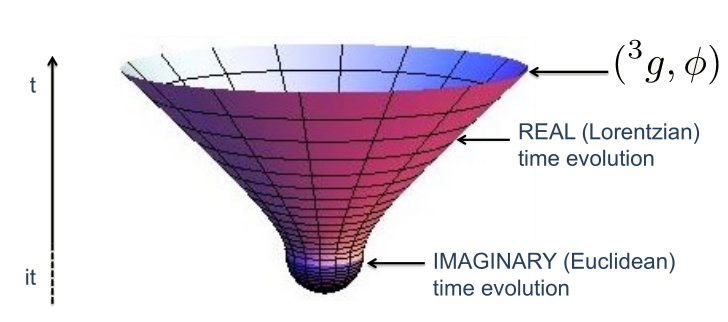
\includegraphics[width=\textwidth]{Universe_Start.png}
    \caption{Sketch of the beginning of the universe}
    \label{fig:UniverseStart}
  \end{figure}
  Now allowing $\tau \in \mathbb{C}$, we can for example choose $\tau = \frac{\pi}{2H} + it$ after some time, giving us
  \begin{equation}
    ds^2 = -\text{d}t^2 + \frac{1}{H^2}\cosh(Ht)^2 \text{d}\Omega_3
  \end{equation}
  I.e the exponentially expanding de-sitter universe that we know, if you stick this complex geometry into the wave-function, and you evaluate this for a large scale factor you get a real part and a phase:
  \begin{equation}
    \Phi[^3g,\phi] \approx A\exp\{iS\}
  \end{equation}
   If you take the final value of the scale factor larger and larger, the phase factor is going to keep increasing $\rightarrow$ wavefunction is going to be oscillating faster and faster, as seen in QFT, this thus becomes classical. 
   I.e we have an Euclidean regime and match it on a lorentzian.
  \\\\
  The real succes of this 'no boundary condition' turns out to be almost one-to-one mappable to the idea of inflation, as intuitively, we need $V(\phi)\gg$ compared to gradients of the field and the kinetic energy for inflation. But we also need this for a no boundary universe as singularities are driven by kinetic en gradient energies contrary to no boundary universes where we can't have that (as we would then have a singularity).
  \section{How to put the wave function to use?}
  The universe could have started with many different $\psi_i$ (the initial value of the scalar field at the bottom of figure \ref{fig:UniverseStart}), illustrated in figure \ref{fig:PossibleStarts}. We need them to start sufficiently high for there to be any inflation.
   \begin{figure}
    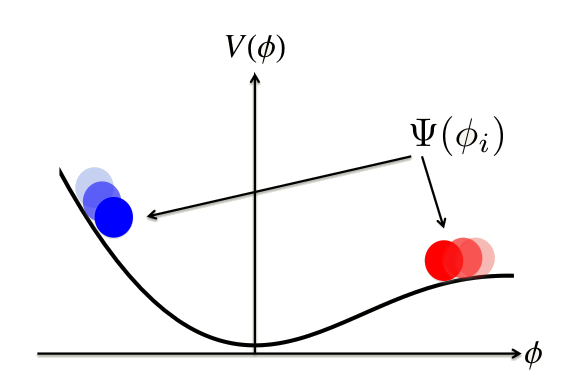
\includegraphics[width=\textwidth]{InitialConditions.png}
    \caption{Sketch of possible starting points for the inflaton field}
    \label{fig:PossibleStarts}
  \end{figure}
  Now, given all we know, what would we expect?
  I.e conditional probability: probability for some observable of CMB: $\Theta_{\text{CMB}}$ given some data about the universe (e.g flat, filled with a certain density of galaxies); $P(\Theta_{\text{CMB}}|\text{data})$. For any question that you're asking there's going to be a whole sum/integral over histories \& universes that exhibit that correlation:
  \begin{equation}
    P(\mathcal{O}|D) \propto \sum_J\int P(D|\mathcal{O},\Phi_i^J)P(\mathcal{O},\Phi_i^J)
  \end{equation}
I.e roughly schematically what this expression means is that you're on one hand (rightmost P) asking for the prior probability for a certain number of e-folds and certain values that come from it (e.g CMB spectra), multiplying by (P just after integral) a factor that accounts for the data $D$ that we already have about the universe. The right factor is pure theory while the left factor (on the RHS) basically summerizes some of the observations we've already done. I.e we're seeking which universe in this huge possibility space dominates the answer, this universes' properties is what the theorist should tell the experimenter. Here you have the pressure of two factors, say e.g if there are not many e-folds, if our data includes data that there're many galaxies around us (high number of e-folds) then the right $P$ pushes it down whilst the left $P$ pushes the number of e-folds up, making it so the combination of the theoretical and observational factor which predicts the dominant history that contributes to the question and thus to which universe we are in.

  \section{Holography}
  You have 2 theories that both claim to be a form of quantum gravity, the classical spacetime extension as seen in the path integral and string theory. 10 years ago the first bridges between string theory and the considered path integral were established, and this has everything to do with the concept known as holography\footnote{the holographic principle is a tenet of string theories and a supposed property of quantum gravity that states that the description of a volume of space can be thought of as encoded on a lower-dimensional boundary to the region}
  In short this amounts to a duality \footnote{i.e 2 languages can describe the same system}  between QFT and gravitational systems. The system in which holography was develepod was in anti-desitter space which has most of it's volume towards the boundaries (see figure \ref{fig:vleermuizen})
  \begin{figure}
    \centering
    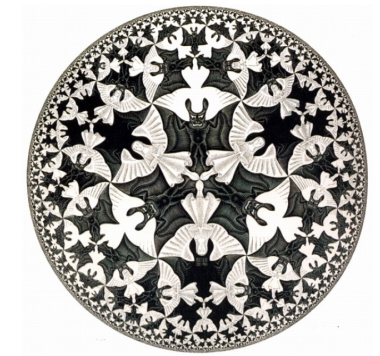
\includegraphics[scale=0.5]{vleermuizen.png}
    \caption{Bats as illustration of anti-desitter space}
    \label{fig:vleermuizen}
  \end{figure}
  Everything that you calculate herein can be re-expressed in terms of a different theory defined on the boundary. This theory is a normal QFT. This is possible because of the fact that most of the volume is near the boundary and that light rays bounce off the boundary. 
  \begin{equation}
    \Psi_{\text{gravity}} \leftrightarrow Z_{QFT}
  \end{equation}
  The theory defined on the boundary is a strong coupled QFT $\rightarrow$ very hard to solve. You get the dimension "back" from the RG (Renormalization group) flow. \\\\
  Now what does this have to do with our wave-function? Whell there is a euclidean version of the holography, which involves euclidean anti-desitter space:
  \begin{equation}
    ds^2 = d\tau^2 + \frac{1}{H^2}\sinh(H\tau)^2\text{d}\Omega_3
  \end{equation}
  This holography says that the wave-function that we've been talking about, which is function of boundary data can be calculated using a QFT defined on the boundary, e.g using a partition function:
  \begin{equation}
    \Psi[^3g,\phi_1] = \mathcal{Z}_{\text{QFT}}[^3g,\alpha]
  \end{equation}
  With $\alpha$ sources of deformation for the lagrangian.\\\\
  Now what does this have to do with inflation? Thinking back to our complex $\tau$ we can do a different route than $\tau = \frac{\pi}{2H} + it$, another way of going is depicted in figure \ref{fig:ADS}.
  \begin{figure}[h]
    \centering
    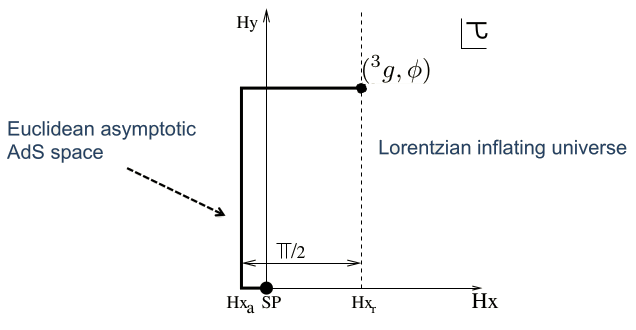
\includegraphics[scale=0.5]{ADS.png}
    \caption{Moving around time so we get an ADS period}
    \label{fig:ADS}
  \end{figure}\\
  These classically different geometries are thus quantum mechanically connected, making it so we can use holography here.
  \begin{figure}
    \centering
    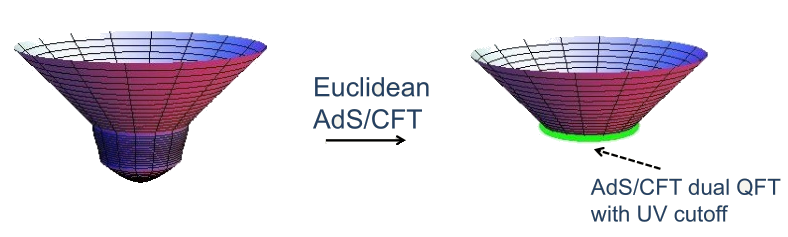
\includegraphics[width=0.8\textwidth]{ADSCFTdual.png}
    \caption{$\Psi \rightarrow \mathcal{Z}_{\text{QFT}}$}
    \label{fig:ridofads}
  \end{figure}
  because of this we can thus get rid of the ADS part as shown in figure \ref{fig:ridofads}.\\\\
  Now remember that in inflationary theory we assumed the fluctuations to be in the ground state (gaussian wave functions), this comes about naturally here as the condition that the geometry is regular selects the inflationary backgrounds and in those backgrounds puts the fluctuations in their ground state.
\end{document}

